\chapter{Literature Review}
\label{cha:review}
In this chapter, I will introduce how solving these kinds of image-to-image
translation tasks with GANs are originated, how the following models trying 
to improve the results by discussing three representative models.
For the two state-of-the-art models(pix2pixHD and SPADE), I will only discuss
the theory here, please check chapter 4 for the implementation details and
results evaluation.

\section{Image-to-Image Translation with cGAN}
Dealing Image-to-Image translation tasks with GANs originated from Isola et al.\cite{pix2pix2016}
which tries to develop a common framework for all “predict pixels from pixels” problems with 
conditional GANs, which shows the ability of generating decent $256 \times 256$ resolution images. 

\subsection{Objective Function}
The objective of our model is to produce photorealistic images that is indistinguishable from the 
real images given input segmentation maps, the cGAN objective function is:
$$\mathcal{L}_{c G A N}(G, D)=\mathbb{E}_{x, y}[\log D(x, y)]+\mathbb{E}_{x, z}[\log (1-D(x, G(x, z))]$$
where the generator G tries to minimize the cGAN loss against an adversarial discriminator D that 
tries to maximize it, i.e. $G^{*}=\arg \min _{G} \max _{D} \mathcal{L}_{c G A N}(G, D)$.
The paper also claims that it is beneficial to mix the GAN objective with a conventional loss 
such as L1 loss: $\mathcal{L}_{L 1}(G)=\mathbb{E}_{x, y, z}\left[\|y-G(x, z)\|_{1}\right]$, so the 
final loss function of our GAN model is:
$$G^{*}=\arg \min _{C} \max _{D} \mathcal{L}_{c G A N}(G, D)+\lambda \mathcal{L}_{L 1}(G)$$
Note in this model, we do not provide noise $z$ like the traditional cGAN does, for we only need 
deterministic results and the random noise is not found helpful in terms of the final outputs.
\begin{figure}[H]
    \begin{center}
    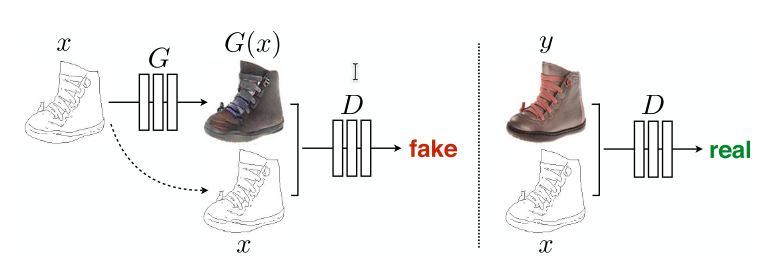
\includegraphics[width=10cm]{figures/pix2pix-cGAN}
    \end{center}
    \caption{cGAN in pix2pix}
    \label{fig:pix2pix-cGAN}
\end{figure}

\subsection{Architecture}
Both the generator and discriminator use modules of the form [CONV2d-BN-ReLU], the 
generator uses a classic encoder-decoder structure where the encoder extracts the 
feature maps from the input segmentation map, and the decoder filled the details 
to produce a photorealistic output from that feature maps. In addition, sharing 
low-level information between input and output is helpful for many image translation
tasks, so in order to shuttle this information across the neural network, the author
adds skip connections following the general structure of a “U-Net”, specifically, we
try to connect each layer $i$ and corresponding layer $n-i$, where $n$ is the total number
of layers, and each skip connections simply concatenates all channels at layer $i$ 
with those at layer $n-i$. For discriminator, the author introduces PatchGAN which 
tries to classify if each $N \times N$ patch in an image is real or fake, this
discriminator has fewer parameters, runs faster, and can be applied to larger images.
\begin{figure}[H]
    \begin{center}
    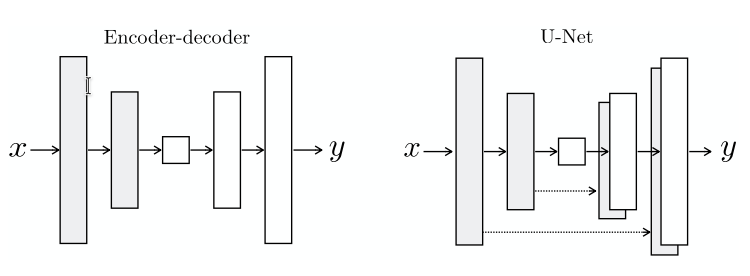
\includegraphics[width=12cm]{figures/pix2pix-generator}
    \end{center}
    \caption{Encoder-decoder generator VS. Skip connections generator}
    \label{fig:pix2pix-generator}
\end{figure}

\subsection{Summary}
The pix2pix model does not require a lot of computation resources, one can easily 
achieve similar results on Google Colab. I ran the official tutorial of image 
translation from Tensorflow2.0 web page, and here are some example outputs after 100
epochs of training on facade dataset\cite{Tylecek13}:
\begin{figure}[H]
    \begin{center}
    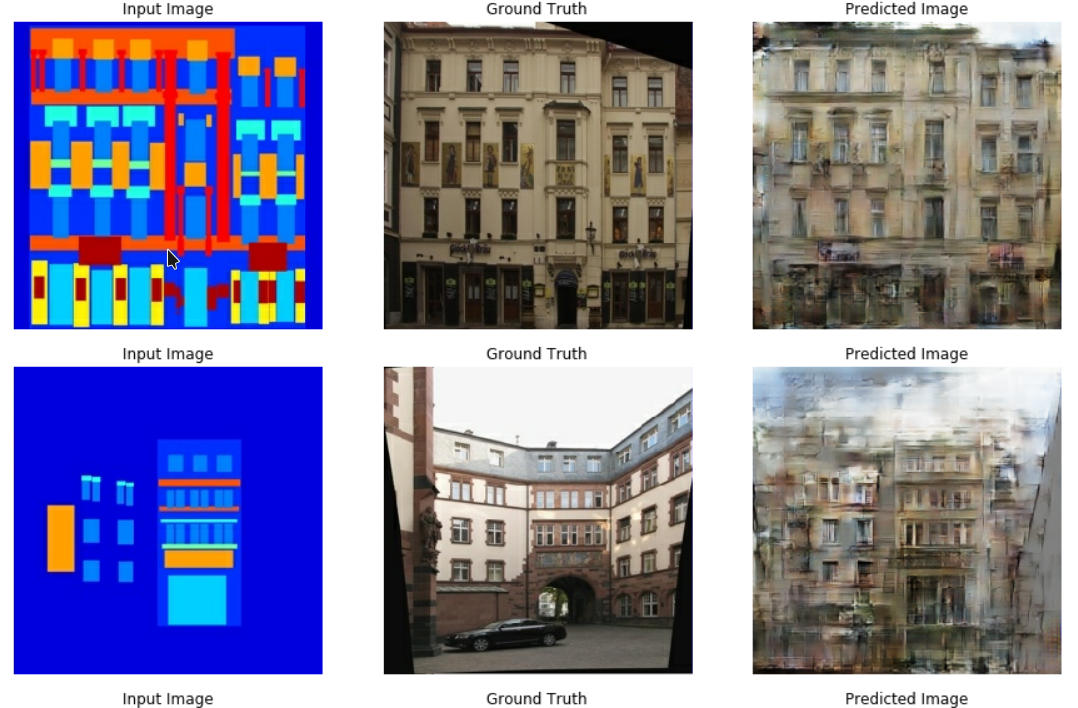
\includegraphics[width=12cm]{figures/pix2pix-output}
    \end{center}
    \caption{Example outputs from pix2pix model}
    \label{fig:pix2pix-output}
\end{figure}

The pix2pix model can achieve decent results with limited computation resources on 
small datasets such as the facade dataset. However, it still cannot produce very
clear textures or high resolution photorealistic images.

\section{State-of-the-art Model — Pix2pixHD}
Pix2pixHD\cite{wang2018pix2pixHD} is the upgraded version of pix2pix brought by 
Nvidia which can generate high resolution images. In the paper they successfully 
generate $2048 \times 1024$ resolution images using the Cityscapes benchmark dataset
\cite{Cordts2016Cityscapes}. The pix2pixHD model is still based on conditional GAN, but
it makes improvements on the generator, the discriminator, and the loss function.

\subsection{Generator}
Generator G consists of two generators, we term G1 as the global generator and G2 as 
the local enhancer. The global generator plays the similar role as the pix2pix model 
which is basically an encoder-decoder generator with residual blocks that can output 
lower resolution($1024 \times 512$) images, and the local enhancer will augment the 
output images to a higher resolution, e.g. $2048 \times 1024$. Both the global generator 
and local enhancer consist of convolution blocks, residual blocks, and transposed convolution blocks,
we named them $G_{1}^{(c)}$, $G_{1}^{(r)}$, $G_{1}^{(t)}$ and $G_{2}^{(c)}$, $G_{2}^{(r)}$, 
$G_{2}^{(t)}$ respectively. In order to integrate the global generator and local enhancer, 
the input to the residual block of the local enhancer is the 
element-wise sum of two feature maps: the output feature map of $G_{2}^{(c)}$, and the last 
feature map of the global generator $G_{1}^{(t)}$. The architecture of the whole generator 
is shown as the following figure:
\begin{figure}[H]
    \begin{center}
    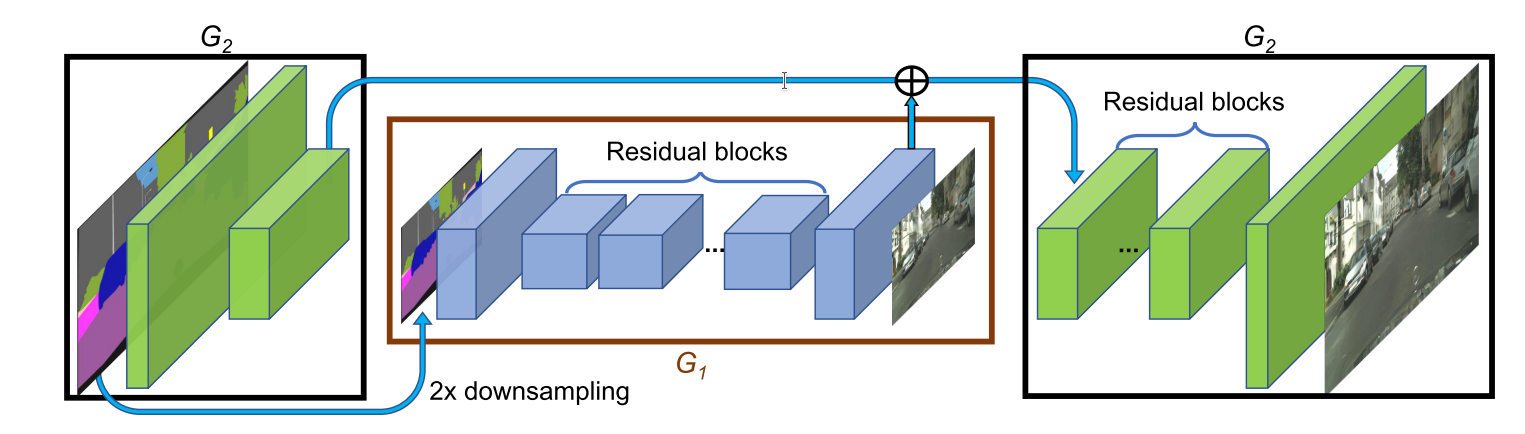
\includegraphics[width=12cm]{figures/pix2pixHD-generator}
    \end{center}
    \caption{Pix2pixHD generator architecture}
    \label{fig:pix2pixHD-generator}
\end{figure}
When training the generator, we need to train the global generator first and then train the 
local enhancer in the order of their resolutions.

\subsection{Discriminator}
Discriminator D is upgraded to Multi-scale discriminators, which alleviate the headache that a 
discriminator needs to have a larger receptive field, i.e. more memory is required, however, we 
all know that memory is already a scarce resource for deep learning models. Therefore, what a 
multi-scale discriminator does is to use 3 smaller discriminators that have identical network
structure but operate at different scales, we named the discriminators as $D_{1}$, $D_{2}$, $D_{3}$ 
respectively. $D_{1}$, $D_{2}$ will deal with the real and synthesized images by factor 2 and 4, 
while $D_{3}$ will deal with the original images. The discriminator that operates at the finest 
scale will focus on the details of an image, while the discriminator that operates at the largest 
scale will have the largest receptive field, discriminating the image with a global view. In 
implementation, we can simply add up the three discriminators' objective functions, which makes 
the learning problem to be:
$$\min _{G} \max _{D_{1}, D_{2}, D_{3}} \sum_{k=1,2,3} \mathcal{L}_{\mathrm{GAN}}\left(G, D_{k}\right)$$

\subsection{Objective Function}
The improved adversarial loss consists of: 
\begin{itemize}
    \item The GAN loss similar to the one in pix2pix model: 
    $$\mathcal{L}_{G A N}(G, D)=\mathbb{E}_{x, y}[\log D(x, y)]+\mathbb{E}_{x}[\log (1-D(x, G(x))]$$
    \item The feature map loss, it is desirable if we can learn to match the intermediate 
    representations from the real and the synthesized image, so in pix2pixHD we extract features 
    from multiple layers of the discriminator and calculate the feature map loss of each layer and 
    then add them up together:
    $$\mathcal{L}_{\mathrm{FM}}\left(G, D_{k}\right)=\mathbb{E}_{(\mathbf{s}, \mathbf{x})} \sum_{i=1}^{T} \frac{1}{N_{i}}\left[\left\|D_{k}^{(i)}(\mathbf{s}, \mathbf{x})-D_{k}^{(i)}(\mathbf{s}, G(\mathbf{s}))\right\|_{1}\right]$$
    Where $D_{k}^{(i)}$ is the i-th layer feature extractor of discriminator $D_{k}$, T is the 
    total number of layers and $N_{i}$ is the number of elements in each layer.
    \item (Optional)VGG loss, also called perceptual loss, we calculate loss with the help of 
    pretrained VGG network\cite{articleVGG}: 
    $\lambda \sum_{i=1}^{N} \frac{1}{M_{i}}\left[\left\|F^{(i)}(\mathbf{x})-F^{(i)}(G(\mathbf{s}))\right\|_{1}\right]$,
    where we choose $\lambda=10$, and $F_{i}$ is the i-th layer with $M_{i}$ elements of 
    the VGG network.
\end{itemize}
The final objective without VGG could be:
$$\min _{G}\left(\left(\max _{D_{1}, D_{2}, D_{3}} \sum_{k=1,2,3} \mathcal{L}_{\mathrm{GAN}}\left(G, D_{k}\right)\right)+\lambda\sum_{k=1,2,3} \mathcal{L}_{\mathrm{FM}}\left(G, D_{k}\right)\right)$$
or including VGG loss:
$$\min _{G}\left(\left(\max _{D_{1}, D_{2}, D_{3}} \sum_{k=1,2,3} \mathcal{L}_{\mathrm{GAN}}\left(G, D_{k}\right)\right)+\lambda\sum_{k=1,2,3} \mathcal{L}_{\mathrm{FM}}\left(G, D_{k}\right) + \lambda \sum_{i=1}^{N} \frac{1}{M_{i}}\left[\left\|F^{(i)}(\mathbf{x})-F^{(i)}(G(\mathbf{s}))\right\|_{1}\right]\right)$$

\section{State-of-the-art Model — SPADE}
Spatially-adaptive (DE)normalization(SPADE)\cite{park2019SPADE} is another upgraded image-to-image 
translation model brought by Nvidia, previous designs including pix2pix \cite{pix2pix2016} and 
pix2pixHD \cite{wang2018pix2pixHD} are based on cGAN structure, which directly feed the semantic 
layout as input to the generator network, then the segmentation map is processed through stacks 
of convolution, batch normalization, residual, non-linearity layers. The paper claims that 
some semantic information get removed by normalization layers, therefore, they proposed a new 
normalization layer which can integrate the information of semantic label maps instead of just 
two trainable parameters in the traditional batch normalization layer. The SPADE borrows the design 
of objective function and discriminator, so we will mainly discuss the generator upgrades next. 
\subsection{SPADE Block}
The SPADE block is the key of SPADE generator, similar to batch normalization, the activation is 
normalized in the channel-wise manner by the following formula:
$$\hat{x}_{i}=\frac{x_{i}-\mu}{\sqrt{\sigma^{2}+\epsilon}} \text { and } y_{i}=\gamma \hat{x}_{i}+\beta$$
Where $x_{i}$ is an activation for the i-th example in the minibatch and $\hat{x}_{i}$ is the output after 
the process, $\mu$ and $\sigma^{2}$ are the mean vlaue and variance of the activation over the batch.
However, in SPADE block, $\gamma$ and $\beta$ are not just 
trainable parameters anymore, they are determined by the input segmentation map, the SPADE block uses
a two-layer convolution module that convert an image into values. Since the important parameters in
this new normalization block are influenced by the input segmentation map, we do not need to worry 
the semantic information being “washed away” during normalization.
\begin{figure}[H]
    \begin{center}
    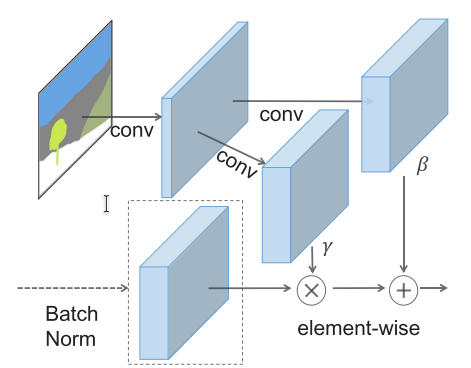
\includegraphics[width=5cm]{figures/SPADE-Block}
    \end{center}
    \caption{Structure of a single SPADE Block}
    \label{fig:SPADE-Block}
\end{figure}

\subsection{SPADE Residual Block}
The SPADE residual block is used to replace the conventional residual block, instead of simply 
using convolutions, it also uses SPADE Block, in this way, we can add the information of the 
input segmentation map into the residual blocks. The structure of a single SPADE residual 
block is as follows:
\begin{figure}[H]
    \begin{center}
    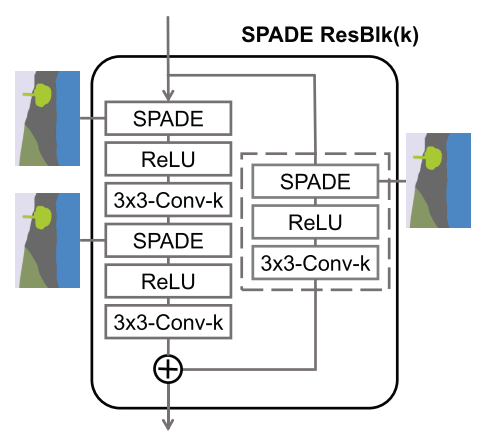
\includegraphics[width=5cm]{figures/SPADE-ResBlock}
    \end{center}
    \caption{Structure of a single SPADE Residual Block}
    \label{fig:SPADE-ResBlock}
\end{figure}

\subsection{Generator}
In order to build a SPADE generator, we need one more step which is to put SPADE residual blocks 
into the structure of a GAN generator. Because we have already put the information of the input 
segmentation map into the residual blocks, we do not need the encoder part of conditional GAN, 
we can just use a random noise as the input like the original GAN models and only keep the 
decoder part. So the structure of the SPADE generator is like the following:
\begin{figure}[H]
    \begin{center}
    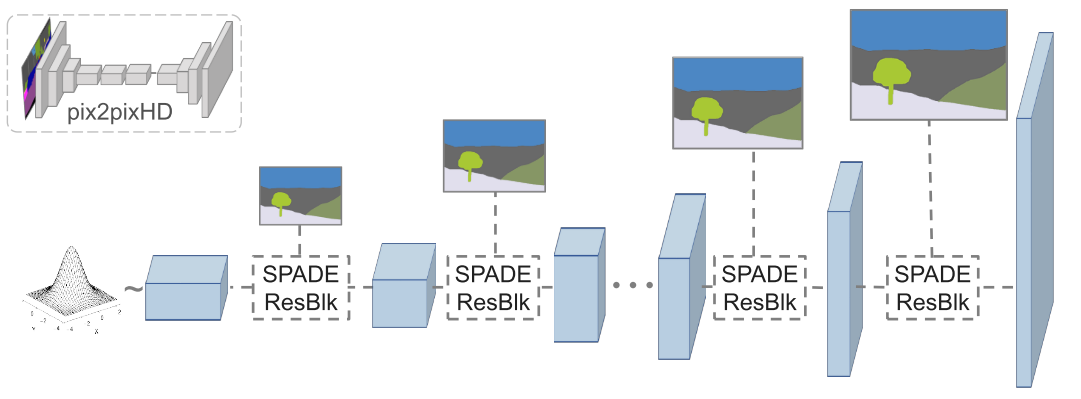
\includegraphics[width=12cm]{figures/SPADE-generator}
    \end{center}
    \caption{Architecture of SPADE generator}
    \label{fig:SPADE-generator}
\end{figure}

\subsection{Other Features}
Apart from the improvement on the generator, SPADE also make some other slight modifications
including changing LSGAN loss in pix2pixHD with 
Hinge loss, applying spectral normalization to the convolution layers in the discriminator.
In addition, since the encoder is no longer necessary to the image transaltion task, SPADE 
allows using a variational auto encoder(VAE) to achieve style transfer. The complete 
architecture of SPADE GAN model is like the following:
\begin{figure}[H]
    \begin{center}
    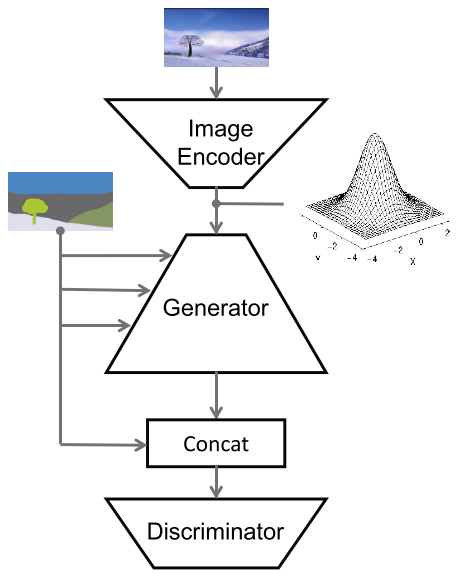
\includegraphics[width=5cm]{figures/SPADE-architecture}
    \end{center}
    \caption{Architecture of SPADE GAN model}
    \label{fig:SPADE-architecture}
\end{figure}
The VAE image encoder encodes a real image to generate a mean and variance which are used 
to further compute the noise that is input to the decoder. The discriminator takes the 
concatenation of the semantic label map and the output image from the generator as input 
and tries to identify whether each image is real or fake.


% Local Variables: 
% mode: latex
% TeX-master: "report"
% End: 
